\documentclass[tikz,border=2pt]{standalone}
\usepackage{amsmath}
\usepackage{pgfplots}
\pgfplotsset{compat=1.18}
\begin{document}
% x_{t+2} - 3x_{t+1} + 2x_t = 0 has the basis y^(1)_t = 1, y^(2)_t = 2^t; the solution with
% x_0 = 5, x_1 = 7 is the combination x_t = 3 y^(1)_t + 2 y^(2)_t = 3 + 2^{t+1} (5, 7, 11, 19).
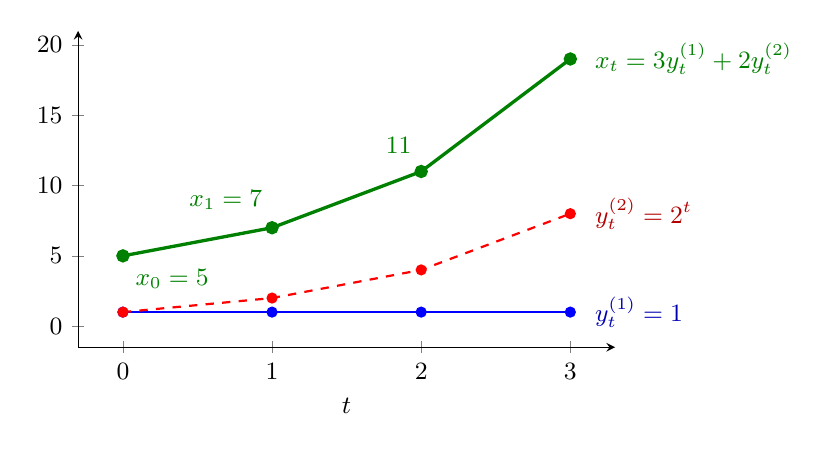
\begin{tikzpicture}[font=\small]
  \begin{axis}[
    axis lines=left, xmin=-0.3, xmax=3.3, ymin=-1.5, ymax=21,
    xtick={0,1,2,3}, ytick={0,5,10,15,20},
    xlabel={$t$}, width=8.4cm, height=5.6cm, clip=false,
    every axis plot/.append style={thick}
    ]
    \addplot[blue, mark=*, mark size=1.6pt] coordinates {(0,1) (1,1) (2,1) (3,1)};
    \addplot[red, dashed, mark=*, mark size=1.6pt, mark options={solid}] coordinates {(0,1) (1,2) (2,4) (3,8)};
    \addplot[green!50!black, very thick, mark=*, mark size=1.8pt] coordinates {(0,5) (1,7) (2,11) (3,19)};
    \node[blue!70!black, anchor=west] at (axis cs:3.1,1) {$y^{(1)}_t=1$};
    \node[red!70!black, anchor=west] at (axis cs:3.1,8) {$y^{(2)}_t=2^t$};
    \node[green!50!black, anchor=west] at (axis cs:3.1,19) {$x_t=3y^{(1)}_t+2y^{(2)}_t$};
    \node[green!50!black, anchor=north west] at (axis cs:0.02,4.7) {$x_0=5$};
    \node[green!50!black, anchor=south east] at (axis cs:1,7.6) {$x_1=7$};
    \node[green!50!black, anchor=south east] at (axis cs:2,11.6) {$11$};
  \end{axis}
\end{tikzpicture}
\end{document}
